
\section{Introduction}
This chapter will describe the observed low energy excess reported by the MiniBooNE and LSND experiments. The LSND experiment first observed an excess of $\overline{\nu}_e$ in a $\overline{\nu}_\mu$ beam in 2001. The MiniBooNE experiment then observed an unexplained excess of electron-like events in a primarily $\nu_\mu$ beam in the neutrino energy region between 200 to 475 MeV in 2009. A description of the LSND observation followed by the MiniBooNE detector and analysis is provided in this chapter. The purpose of this chapter is to provide a historical motivation for the eventual sensitivity studies done for the MicroBooNE experiment, which will be described in Chapter \ref{sec:LEEsensitivity}.\\

\section{LSND Observation}
%Brief discussion of the LSND experiment and how they saw an excess of antinue in the antinumu beam with L/E that didn't fit in with any measured mixing angles and delta m2 in 3 neutrino model.

In 2001, the Liquid Scintillator Neutrino Detector (LSND) collaboration published an observation of excess events consistent with $\overline{\nu}_e$ interactions above the expected background in a $\overline{\nu}_\mu$ beam at the Los Alamos Neutron Science Center \cite{LSNDPaper}. Given the $\frac{L}{E}$ ($\approx$ $\frac{30 m}{40 MeV}$) for this measurement, the excess disagreed with previous measurements of neutrino mixing angles and $\Delta m^2$ values in the three neutrino model. The LSND excess corresponded to a $\Delta m^2$ of approximately 1 $eV^2$, orders of magnitude higher than previously measured values of $\Delta m_{12}^2$ and $\Delta m_{23}^2$. One explanation for this drastically different $\Delta m^2$ value is the possible existence of potential additional ``sterile'' neutrino states, which must not interact weakly given the Z- boson decay width constrains the number of weakly interacting neutrino states to three.\\

To test the LSND result, the MiniBooNE experiment was designed. It would measure $\nu_e$ interactions in a primarily $\nu_\mu$ beam, with a similar $\frac{L}{E}$ ($\approx$ $\frac{500m}{700 MeV}$).


\section{The MiniBooNE Experiment}

\subsection{The MiniBooNE Detector and Monte Carlo Simulation}

%Description of the detector, a schematic figure, description of cherenkov rings, the location of the detector in the BNB. Discussion of how they use NUANCE, mention they use identical beam simulation and reweighting (reweighting should be covered in the beam chapter).


The MiniBooNE detector \cite{MBDetectorPaper} consists of a spherical tank located 541 meters downstream of the BNB neutrino production target, with diameter of 12.2 meters filled with 818 tons of mineral oil underneath at least 3 meters of earth overburden as shown in Figure \ref{MB_detector_fig}. There exists a signal region instrumented with 1280 8-inch photomultiplier tubes (PMTs), most of which were reused from the LSND experiment, and a 35 cm thick outer veto region separated by an opaque barrier instrumented with 240 PMTs. The efficiency for rejecting cosmic ray muons by using with the outer veto region was measured to be 99.99\%.\\
%As seen in the figure, there exists an opaque barrier separating a veto region and a signal region.In the signal region, the photocathode coverage is 11.8\%. This region is intended to identify beam neutrino interactions happening within it; the PMTs face radially inwards. The veto region is 35 cm thick and is instrumented with 240 PMTs which face tangent to the detector radius and its purpose is to reject backgrounds coming from outside of the detector (cosmics, which have a rate at the detector location of about 10 kHz). The inner surface of the veto region is coated in a reflective paint.  
\begin{figure}[ht!]
\centering
	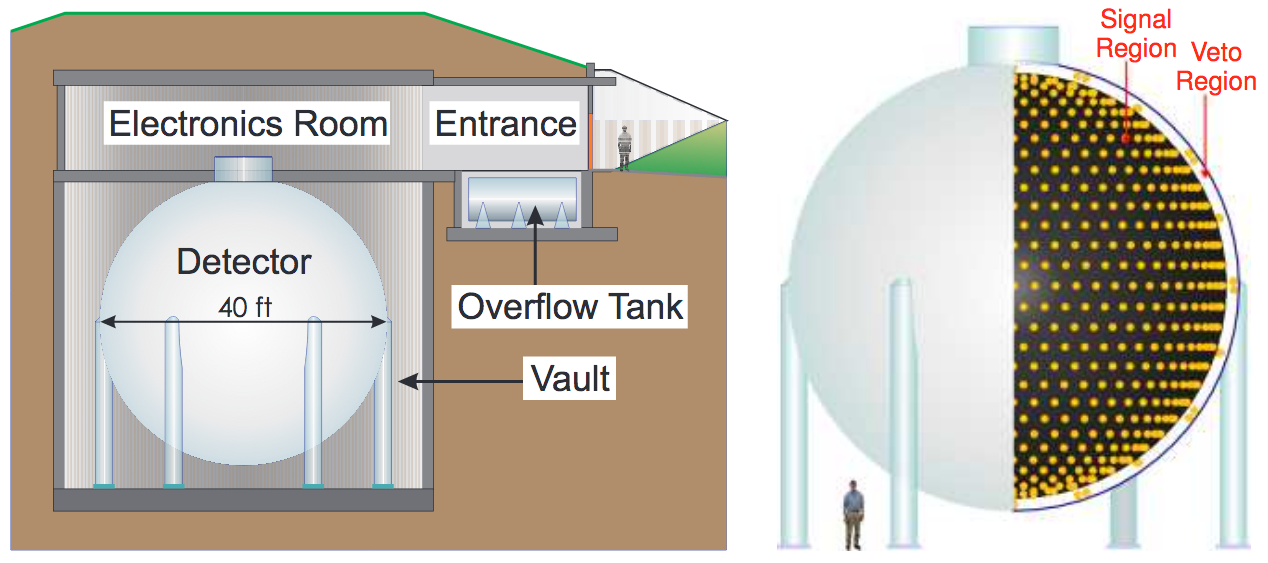
\includegraphics[width=0.9\textwidth]{Figures/MB_detectorpaper_fig.png} \\
\caption{\textit{The MiniBooNE detector enclosure (left) and a cut-away drawing (right) of the detector showing the distribution of PMT's in the signal and veto regions.}}\label{MB_detector_fig}
\end{figure}

The detection method of the MiniBooNE experiment is based primarily on Cherenkov light. The mineral oil within the signal region acts as the neutrino target material.  The majority of final state particles exiting neutrino interactions at neutrino energies from the BNB are produced above Cherenkov threshold. These particles produce Cherenkov light which is detected by the PMTs lining the signal region of the detector. Reconstructing the pattern this light projects onto the walls of the signal region allows for some particle identification abilities.\\

% The PMTs have a wavelength dependent efficiency with a peak at 390 nm, with half that efficiency at 315 and 490 nm. They are operated at +2000 V which results in a gain of approximately $1.6 \times 10^7$. They have an intrinsic time resolution on the order of 1 ns, which is the dominant contribution to the final time resolution in the final PMT data after readout through data acquisition (DAQ) electronics. The DAQ reads out a PMT when the charge signal corresponds to more than 0.1 photoelectrons (PE). The dead time between successive PMT readouts is on the order of 250 ns after the first readout began. PMT charge and timing information is stored in intervals of 200 $\mu s$ following any trigger signal. The trigger signal of interest for this analysis is the beam trigger which is induced by the BNB accelerator clock such that the DAQ begins readout 5 $\mu s$ before each beam spill.\\


%The mineral oil used in MiniBooNE is Marcol 7 Light Mineral Oil ($CH_2$). While the oil has lower density than water (a common material choice for Cherenkov detectors) and therefore smaller probability of a neutrino interacting within the detector, the other benefits outweigh this downside. The oil has good light transmission throughout the wavelength range of 320 nm to 600 nm, relatively large refractive index (1.47, greater than water at 1.33), and its long extinction length of greater than 20 m for 420 nm light. This extinction length allows for loss of no more than 25\% of light generated by a neutrino interaction at the center of the detector. Additionally, the Cherenkov threshold is lower than that of water for the final state particles of interest (electrons, pions, muons, protons), allowing for the measurement of lower energy particles.\\

The detector is calibrated with a series of \textit{in situ} measurements, primarily with cosmic ray muons. Cosmic ray muons stopping within the detector along with an external muon hodoscope provide for angular resolution measurements. Additionally, muons which stop and produce decay electrons that have a known energy endpoint of around 50 MeV provide an energy calibration source at low energies, while through-going muons provide calibration information at higher energies. Also, tagged $\pi^0$ particles which decay into two photons have a known mass of around 135 MeV and therefore provide energy calibration information in that region.\\

\subsection{MiniBooNE Event Selection}
% Brief description of their event selection cuts, mention that the energy definition they use is CCQE and they're looking specifically for CCQE topologies, description of what CCQE means. Figure of their results indicating the excess in neutrino mode. 

Different final state particles exiting a neutrino interaction in the MiniBooNE signal volume create different patterns of Cherenkov light read out by the PMTs. Figure \ref{georgia_cherenkov_cartoon_fig} \cite{GeorgiaThesis} shows how these patterns differ for different common kinds of final state particles (muons, electrons/photons, and neutral pion decays). A muon track produces a crisp, filled-in ring of Cherenkov light, while an electron or photon produces a more fuzzy, hollow ring. A neutral pion decay will result in two photons. By reconstructing these patterns in the PMT data read out from a triggered event in MiniBooNE, the flavor and energy of the interacting neutrino can be determined. With this kind of detection technique it is important to note that a single photon signal is indistinguishable from that of a single electron signal, a fact leading to the ultimate ambiguity of the observed low energy excess in MiniBooNE.\\

\begin{figure}[ht!]
\centering
	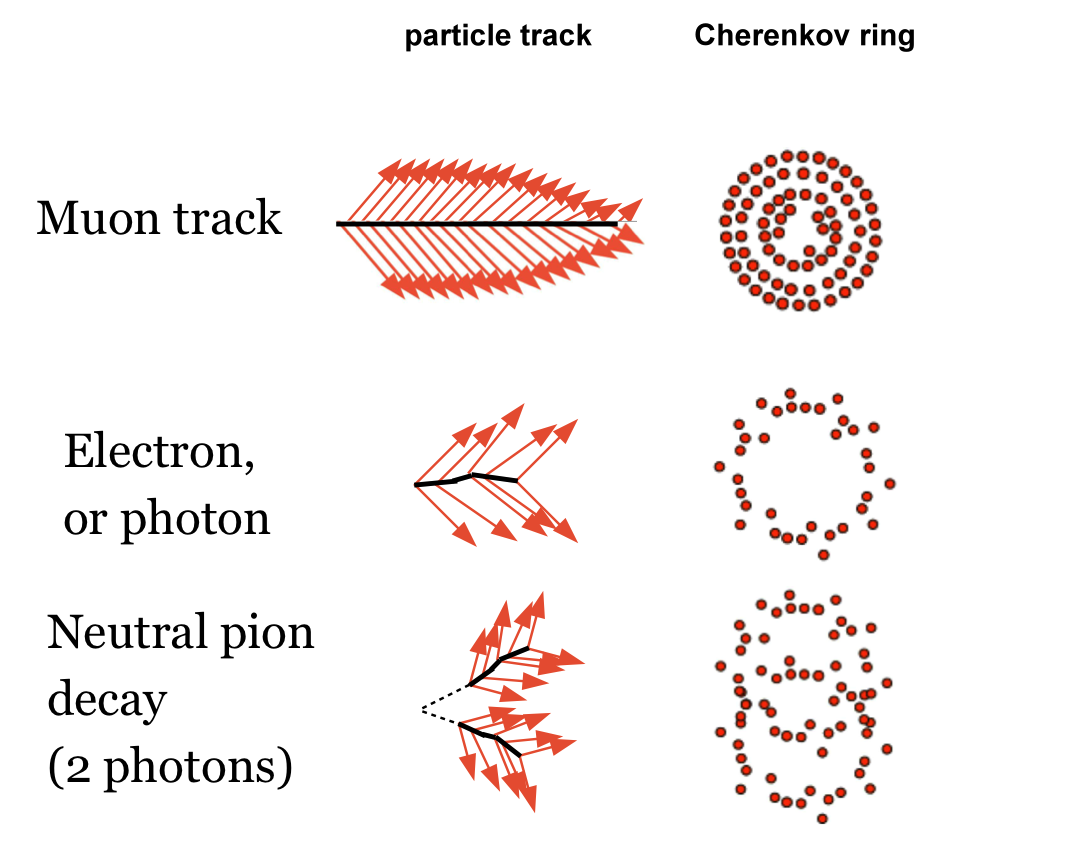
\includegraphics[width=0.9\textwidth]{Figures/georgia_cherenkov_cartoon.png} \\
\caption{\textit{A schematic of the pattern Cherenkov light from different particles would make projected onto the inner walls of the MiniBooNE detector. Top is a muon track (a filled-in ring), middle is an electron (a fuzzy ring), bottom is a photon that pair-produces and creates two fuzzy rings.}}\label{georgia_cherenkov_cartoon_fig}
\end{figure}

The topology of interest in the MiniBooNE oscillation search is that of charged-current quasi-elastic (CCQE) interactions, shown in Figure \ref{georgia_ccqe_feynman_fig}. This interaction channel is the dominant one in the neutrino energy range of the BNB, around 1 GeV $E_\nu$. In a $\nu_l$ CCQE interaction (where $l$ is the neutrino flavor), a lepton of flavor $l$ is produced, along with a proton. The single outgoing lepton is the characteristic event signature for which MiniBooNE searches.\\


\begin{figure}[ht!]
\centering
	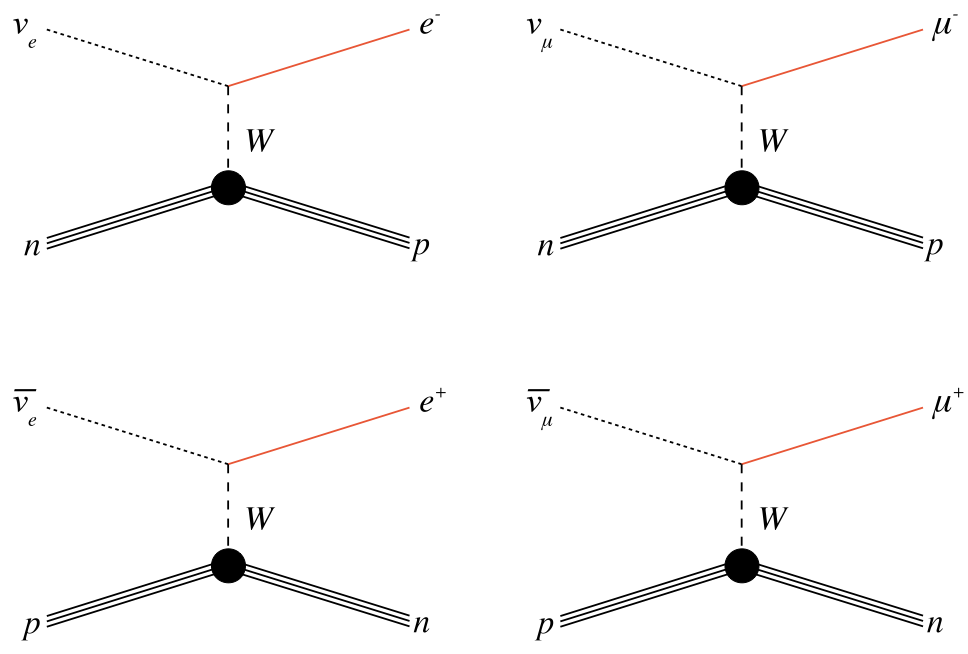
\includegraphics[width=0.9\textwidth]{Figures/georgia_ccqe_feynman.png} \\
\caption{\textit{Feynman diagrams of the charged-current quasi-elastic (CCQE) interaction channel for $\nu_e$, $\nu_\mu$, $\overline{\nu_\mu}$, and $\overline{\nu_e}$ (clockwise from the top left). $\nu_e$ CCQE is the signal channel for the MiniBooNE oscillation analysis.}}\label{georgia_ccqe_feynman_fig}
\end{figure}


In order to select $\nu_e^{CCQE}$ events, cuts are placed to mitigate backgrounds. The most powerful rejection comes from requiring the events occur within the beam timing window. The beam arrives at the detector at a rate of 5 Hz, and each spill lasts 1.6 $\mu s$ and is composed of approximately 80 buckets separated by 19 $ns$. Given the time scale with which MiniBooNE measures the light from interactions, cuts on event timing alone reduces non-beam backgrounds to $\sim10^{-3}$. Two additional cuts are used that require there be more activity within the signal volume than the outer veto volume, a signature characteristic of beam related neutrino events. These pre-cuts achieve more than a 99.99\% rejection of beam unrelated backgrounds. The efficiency to select $\nu_e^{CCQE}$ events in MiniBooNE depends on which cuts are applied in the analysis, but varies between 55\% (with a purity of 36.8\%) and 26.6\% (with a purity of 77.0\%)\cite{MB_numueff_source}. The efficiency to select $\nu_e^{CCQE}$ events also depends on which cuts are applied but varies between 55.2\% and 30.6\%\cite{MB_nueeff_source}.\\

In order to reconstruct events, MiniBooNE uses a maximum likelihood fitting algorithm leveraging properties of charged particle tracks inferred from measured charges and times on the PMTs. The likelihoods to different event hypothesis are used to classify each event as a signal $\nu_e$ CCQE event, or as a background process like $\nu_\mu$ CCQE and NC $\pi^0$ production. Note that MiniBooNE cannot differentiate between a $\mu^+$ and a $\mu^-$, or $e^+$ and $e^-$ so discrimination between neutrino and antineutrino on an event-by-event basis is impossible.\\

Assuming CCQE kinematics, the incident neutrino energy is reconstructed with knowledge of the outgoing lepton energy ($E_l$) and scattering angle ($\theta_l$). In MiniBooNE specifically, the struck nucleon is assumed to be at rest, so the incident neutrino energy $E_\nu^{CCQE}$ is given by:
\begin{equation}\label{MB_CCQE_formula}
E_\nu^{CCQE} = \frac{2m_nE_l+m_p^2-m_n^2-m_l^2}{2(m_n-E_l+\cos\theta_l\sqrt{E_l^2-m_l^2})}
\end{equation}
where $m_n$, $m_p$, $m_l$ are the masses of the neutron, proton, and lepton respectively, and $\theta_l$ is the scattering angle of the outgoing lepton with respect to the (known) beam neutrino direction.\\

\subsection{MiniBooNE Results}
%http://www-boone.fnal.gov/slides-talks/conf-talk/shaevitz/shaevitz-lownu.pdf
%http://www-boone.fnal.gov/slides-talks/conf-talk/zdjurcic/Djurcic_MiniBooNE_NuFact2010.pdf
With the described reconstruction methods and energy definition, the MiniBooNE published results \cite{MBLEEPaper} for the $\nu_e$ appearance search in neutrino mode running are shown in Figure \ref{MB_published_stackedhisto_fig}. Note that besides the irreducible intrinsic $\nu_e$ backgrounds, the dominant background in the excess region is $\pi^0$ mis-identification (MID) (red). In a $\pi^0$ MID event event, a $\pi^0$ is created in the neutrino interaction and its subsequent immediate decay into two photons mimics a the $\nu_e$ CCQE signature (either one photon escapes, or rings overlap). Another important background is $\Delta\rightarrow N\gamma$ (brown). Recall that both of these backgrounds arise from MiniBooNE's inability to distinguish electrons from photons, an important ambiguity which will be discussed in more detail in the following sections.\\


\begin{figure}[ht!]
\centering
	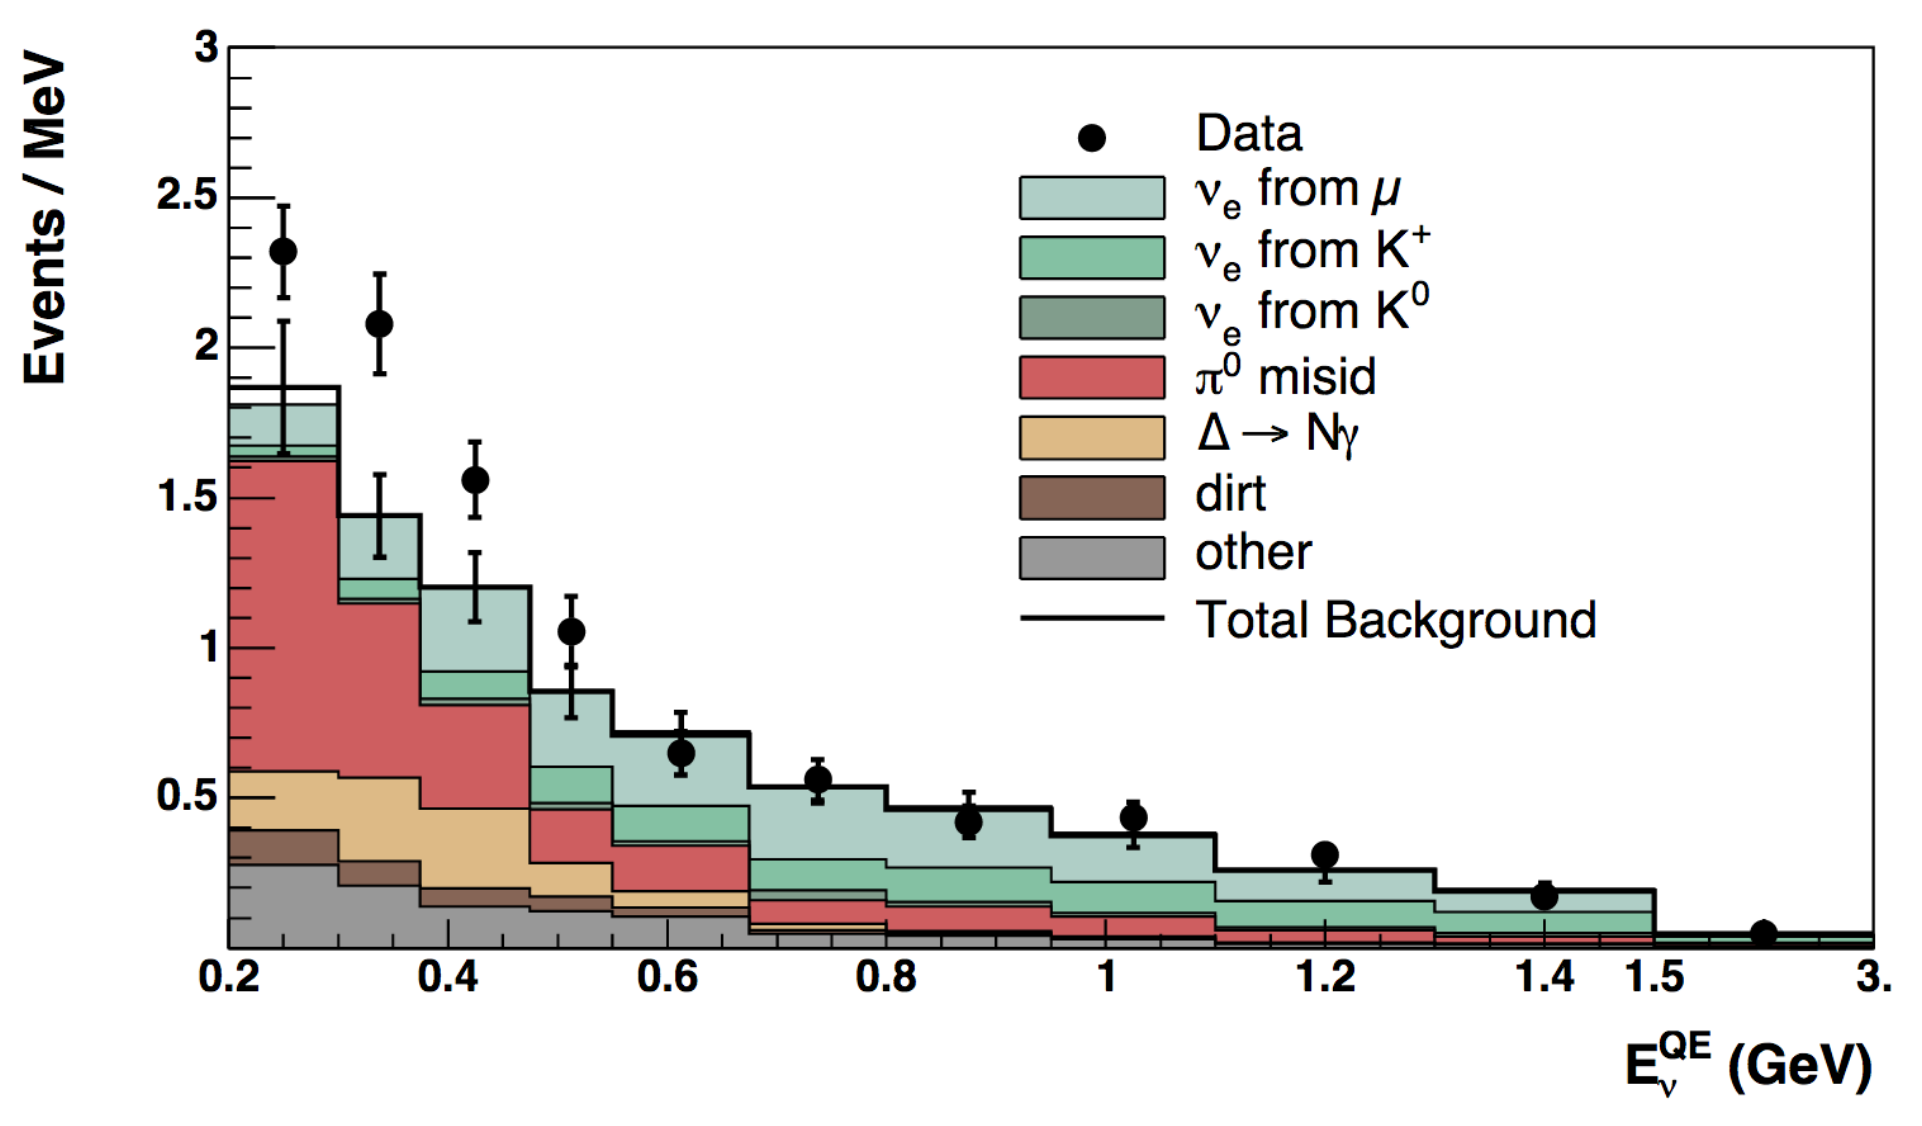
\includegraphics[width=0.9\textwidth]{Figures/MB_published_stackedhisto.png} \\
\caption{\textit{The $E_\nu^{QE}$ distribution for MiniBooNE data (points with statistical errors) and and backgrounds (histogram with systematic errors).}}\label{MB_published_stackedhisto_fig}
\end{figure}


As shown in Figure \ref{MB_published_stackedhisto_fig}, in the energy region $E_\nu^{QE} > 475$ MeV there is good agreement between data and background prediction, making a two neutrino fit inconsistent with the LSND results at the 98\% confidence level assuming CP conservation. Meanwhile, below $E_\nu^{CCQE}$ of 475 MeV there is a statistically significant (6$\sigma$, reduced to 3$\sigma$ after systematics) excess. The excess of 129 $\pm$ 43 events (stat+syst) is consistent in magnitude with the LSND oscillations.\\


In a later separate antineutrino run (in which the BNB horn current is switched to produce a primarily $\overline{\nu}_\mu$ beam), an excess was observed in the energy region $E_\nu^{QE} > 475$ MeV that was consistent with an LSND-type two neutrino oscillation over the null oscillation hypothesis at the 91\% confidence level. In the lower energy region $E_\nu^{QE} < 475$ MeV, an excess of 38.6 $\pm$ 18.5 events was observed. In a fit to the full energy range $E_\nu^{QE} > 200$ MeV, the excess was consistent with an LSND-type two neutrino oscillation over the null oscillation hypothesis at the 98\% confidence level.\\


\subsection{Proposed Low Energy Excess Sources}

% The LEE could either be electron like or photon like, MiniBooNE couldn't tell. Mention of theories like sterile neutrinos though no models seem to fit very well (3+1 or 3+2 with possible CP violation), single photon background misestimations or unexpected backgrounds, neutrino decay, lorentz violation etc etc. 
Shown in Figure \ref{MB_published_excess_fits_fig} is the MiniBooNE neutrino mode excess (data - expected background) with oscillation fits with parameters constrained to be in the LSND allowed region. The parameters in the LSND allowed region are ruled out at the 95\% confidence level if the data are fit with $E_\nu^{CCQE}>$ 475 MeV. \\

\begin{figure}[ht!]
\centering
	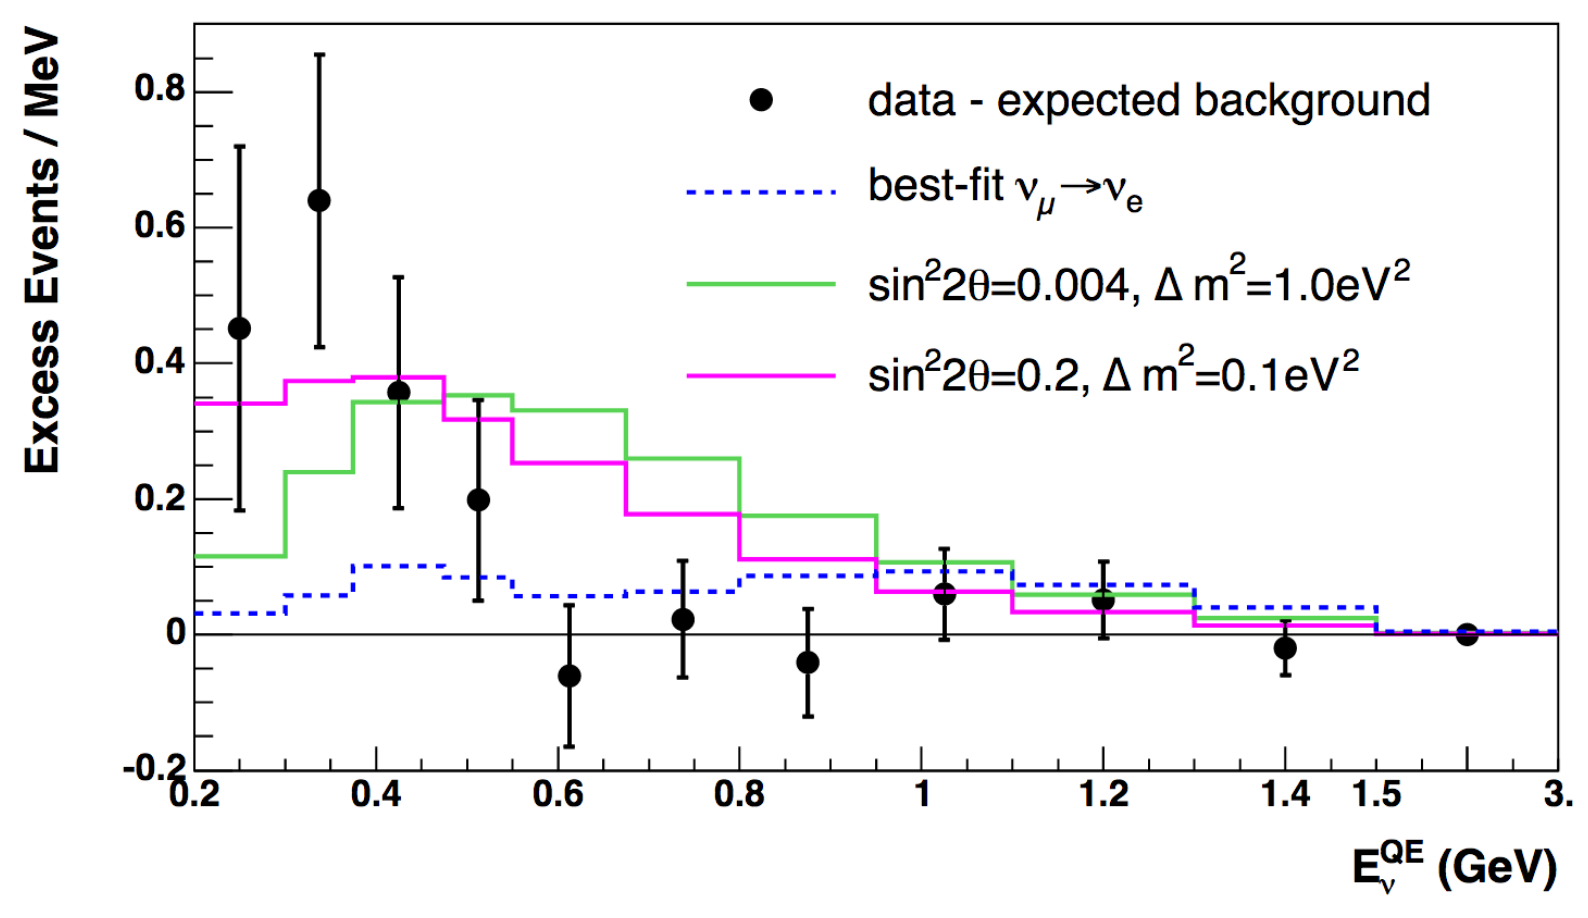
\includegraphics[width=0.9\textwidth]{Figures/MB_published_excess_fits.png} \\
\caption{\textit{The MiniBooNE event excess as a function of $E_\nu^{QE}$. Also shown are the expectations from the best oscillation fit and from neutrino oscillation parameters in the LSND allowed region. The error bars include both statistical and systematic errors.}}\label{MB_published_excess_fits_fig}
\end{figure}

Given MiniBooNE's inability to distinguish electrons from photons, the origin of this excess is either a mis-estimation of one of the backgrounds, or some sort of new physics. The former is unlikely the case because MiniBooNE makes many \textit{in situ} measurements that allow for the constraining of these backgrounds. The neutral current induced backgrounds (NC $\pi^0$, $\Delta\rightarrow N\gamma$, and dirt) are constrained by such measurements. Measurements constraining these backgrounds are described in more detail in the following paragraphs.\\

The NC $\pi^0$ rate in MiniBooNE is measured by selecting events with reconstructed mass near the $\pi^0$ mass. This obtains a $>90$\% pure sample of NC $\pi^0$ interactions which is compared to simulation to obtain a correction function in order to bring the simulated distribution in agreement with data. This same correction function is applied to NC $\pi^0$ events that are backgrounds in the $\nu_e$ appearance analysis. This correction function increases the NC $\pi^0$ background by less than 13\% for $E_\nu^{CCQE}$ $<$ 400 MeV and decreases the background by as much as 20\% above this neutrino energy region. Including this correction factor, the uncertainty on the overall NC $\pi^0$ backgrounds is 7\%. Note that a correction factor of 2.0 would be required to explain the origin of the excess as originating from a mis-estimated NC $\pi^0$ background \cite{GeorgiaThesis}.\\

The excess is unlikely caused by a mis-estimation of the $\Delta\rightarrow N\gamma$ backgrounds because they are additionally constrained by the NC $\pi^0$ measurement through the relative rate of resonant production times a branching fraction of (0.56$\pm$0.04)\%. With this measurement, the uncertainty on the $\Delta\rightarrow N\gamma$ backgrounds is 12\%. Note that a (very large) correction factor of 2.7 would be required to explain the origin of the excess as originating from a mis-estimated $\Delta \rightarrow N\gamma$ background.\\

The excess is unlikely caused by a mis-estimation of the dirt backgrounds because a direct measurement is made by selecting a separate event sample which are likely dirt events and comparing data to simulation. These events are reconstructed close to the detector boundaries with direction pointed generally inwards. In neutrino mode, a dirt background normalization correction factor was computed to be 0.7 $\pm$ 0.1 (with simulation over-predicting the dirt rate normalization). Given the power of the event selection cuts designed to mitigate dirt backgrounds, the relevance of this relatively large correction factor is minimal.\\

The charged current induced backgrounds (intrinsic $\nu_e^{CCQE}$) are reduced with \textit{in situ} measurements of $\nu_\mu$CCQE interactions. A data to simulation comparison of measured $\nu_\mu$CCQE interactions allows for the retuning of underlying flux and cross section parameters in order to bring simulated distributions in agreement with data. These parameters are the same as those used to predict the $\nu_e^{CCQE}$ rate and shape. In addition, a measurement of the highest energy $\nu_\mu$CCQE interactions allows for the further constraint of $\nu_e^{CCQE}$ from kaon decay backgrounds, which is discussed in more detail in a later section of this thesis.\\

Given the likelihood that the excess is not caused by misidentified backgrounds, several new-physics interpretations have been proposed in attempt to explain the excess, including sterile neutrino oscillations (with one, two, or more sterile neutrinos), and new interactions both within and outside of the standard model (CPT violation, quantum decoherence, sterile neutrino decay, etc). A summary of these interpretations can be found in \cite{MBLEESourcesOverview}. A commonality between all interpretations is that their interactions pass the MiniBooNE event selection cuts; that is, they have one electron or one photon exiting the interaction vertex.\\

\section{Conclusions}
This chapter has presented the historical background of the ``low energy excess'', initially observed by the LSND experiment in 2001, then later observed by the MiniBooNE experiment with final analysis published in 2009. Possible sources for this excess have been discussed, including mis-estimated backgrounds and sterile neutrinos, among other things. Ultimately the excess as seen by MiniBooNE can be attributed to an excess of either electron-like events, or photon-like events. Determining which case is beyond the capabilities of MiniBooNE due to limitations of its detector technology (Cherenkov). Because of this limitation, the MicroBooNE experiment was proposed in 2007 ~\cite{MicroBooNEProposal}. This experiment would measure the same neutrino beam in a similar location as MiniBooNE, but would use a detector technology with electron/photon separation powers (liquid argon time projection chambers) to search for and clarify the ambiguity in this excess. The detailed analysis aimed to quantify the sensitivity to a specifically electron-like MiniBooNE excess in the MicroBooNE detector is the subject of the following chapter of this thesis.